% Problem Set 2: Volatility. Compile with: pdflatex volatility_ps.tex (run twice).
% Figures are produced by volatility_ps.py; all numbers are in results.json.
\documentclass[11pt]{article}
\usepackage[letterpaper,margin=1in]{geometry}
\usepackage[T1]{fontenc}
\usepackage{lmodern}
\usepackage{amsmath,amssymb}
\usepackage{booktabs}
\usepackage{graphicx}
\usepackage[font=small,labelfont=bf]{caption}
\usepackage{xcolor}
\usepackage{titlesec}
\usepackage{enumitem}
\setlist[itemize]{topsep=2pt,itemsep=3pt,parsep=0pt}
\usepackage[hidelinks]{hyperref}

\titleformat{\section}{\large\bfseries}{}{0pt}{}
\titleformat{\subsection}{\normalsize\bfseries}{}{0pt}{}
\setlength{\parindent}{0pt}
\setlength{\parskip}{6pt}
\renewcommand{\topfraction}{0.9}
\renewcommand{\bottomfraction}{0.8}
\renewcommand{\textfraction}{0.1}
\renewcommand{\floatpagefraction}{0.8}

\newcommand{\E}{\mathbb{E}}
\newcommand{\1}{\mathbf{1}}

\title{\textbf{Problem Set 2: Volatility}}
\author{MGT 927}  % add your name here
\date{}

\begin{document}
\maketitle
\vspace{-1.5em}

We use daily CRSP data from WRDS for 2 January 1990 to 31 December 2020, which gives 7,812
trading days. The market series is the CRSP value-weighted return (\texttt{vwretd}) and MSFT
is its CRSP holding-period return, both in percent per day. We code every likelihood by hand
and maximize it numerically. Standard errors are the Bollerslev--Wooldridge robust sandwich,
and the point estimates agree with the \texttt{arch} Python package to three decimals. The
code is in \texttt{volatility\_ps.py}.

\begin{center}
\small
\begin{tabular}{lrrrrrrr}
\toprule
 & Mean & S.d. & Ann.\ vol & Skew & Excess kurt. & Min & Max \\
\midrule
Market & 0.044 & 1.13 & 17.9\% & $-0.32$ & 11.0 & $-11.8$ & 11.5 \\
MSFT   & 0.102 & 2.02 & 32.1\% & 0.23 & 6.5 & $-15.6$ & 19.6 \\
\bottomrule
\end{tabular}
\end{center}

%=====================================================================
\section{Question 1}

\subsection{(a) Autocorrelations of returns and squared returns}

Before looking at the data we expected the market to show the stronger volatility clustering.
Write MSFT's return as $r_{i,t}=\beta r_{m,t}+e_{i,t}$. The part of volatility that persists
for weeks or months comes from economy-wide conditions such as recessions, financial stress
and uncertainty about policy, and the index is exposed to all of it. MSFT carries the same
market component plus firm-specific news: earnings announcements, product news and, in this
sample, an antitrust case. That kind of news tends to arrive as a single large move that is
not followed by more large moves. Each such day adds a big value of $r_{i,t}^2$ that has no
counterpart in the days around it, so it raises the variance of squared returns without
raising their autocovariance, and the measured autocorrelation falls. Diversification strips
this component out of the index. For returns themselves we expected autocorrelations close to
zero in both series, since predictable daily returns in liquid stocks would be traded away.

\begin{figure}[!htb]
\centering
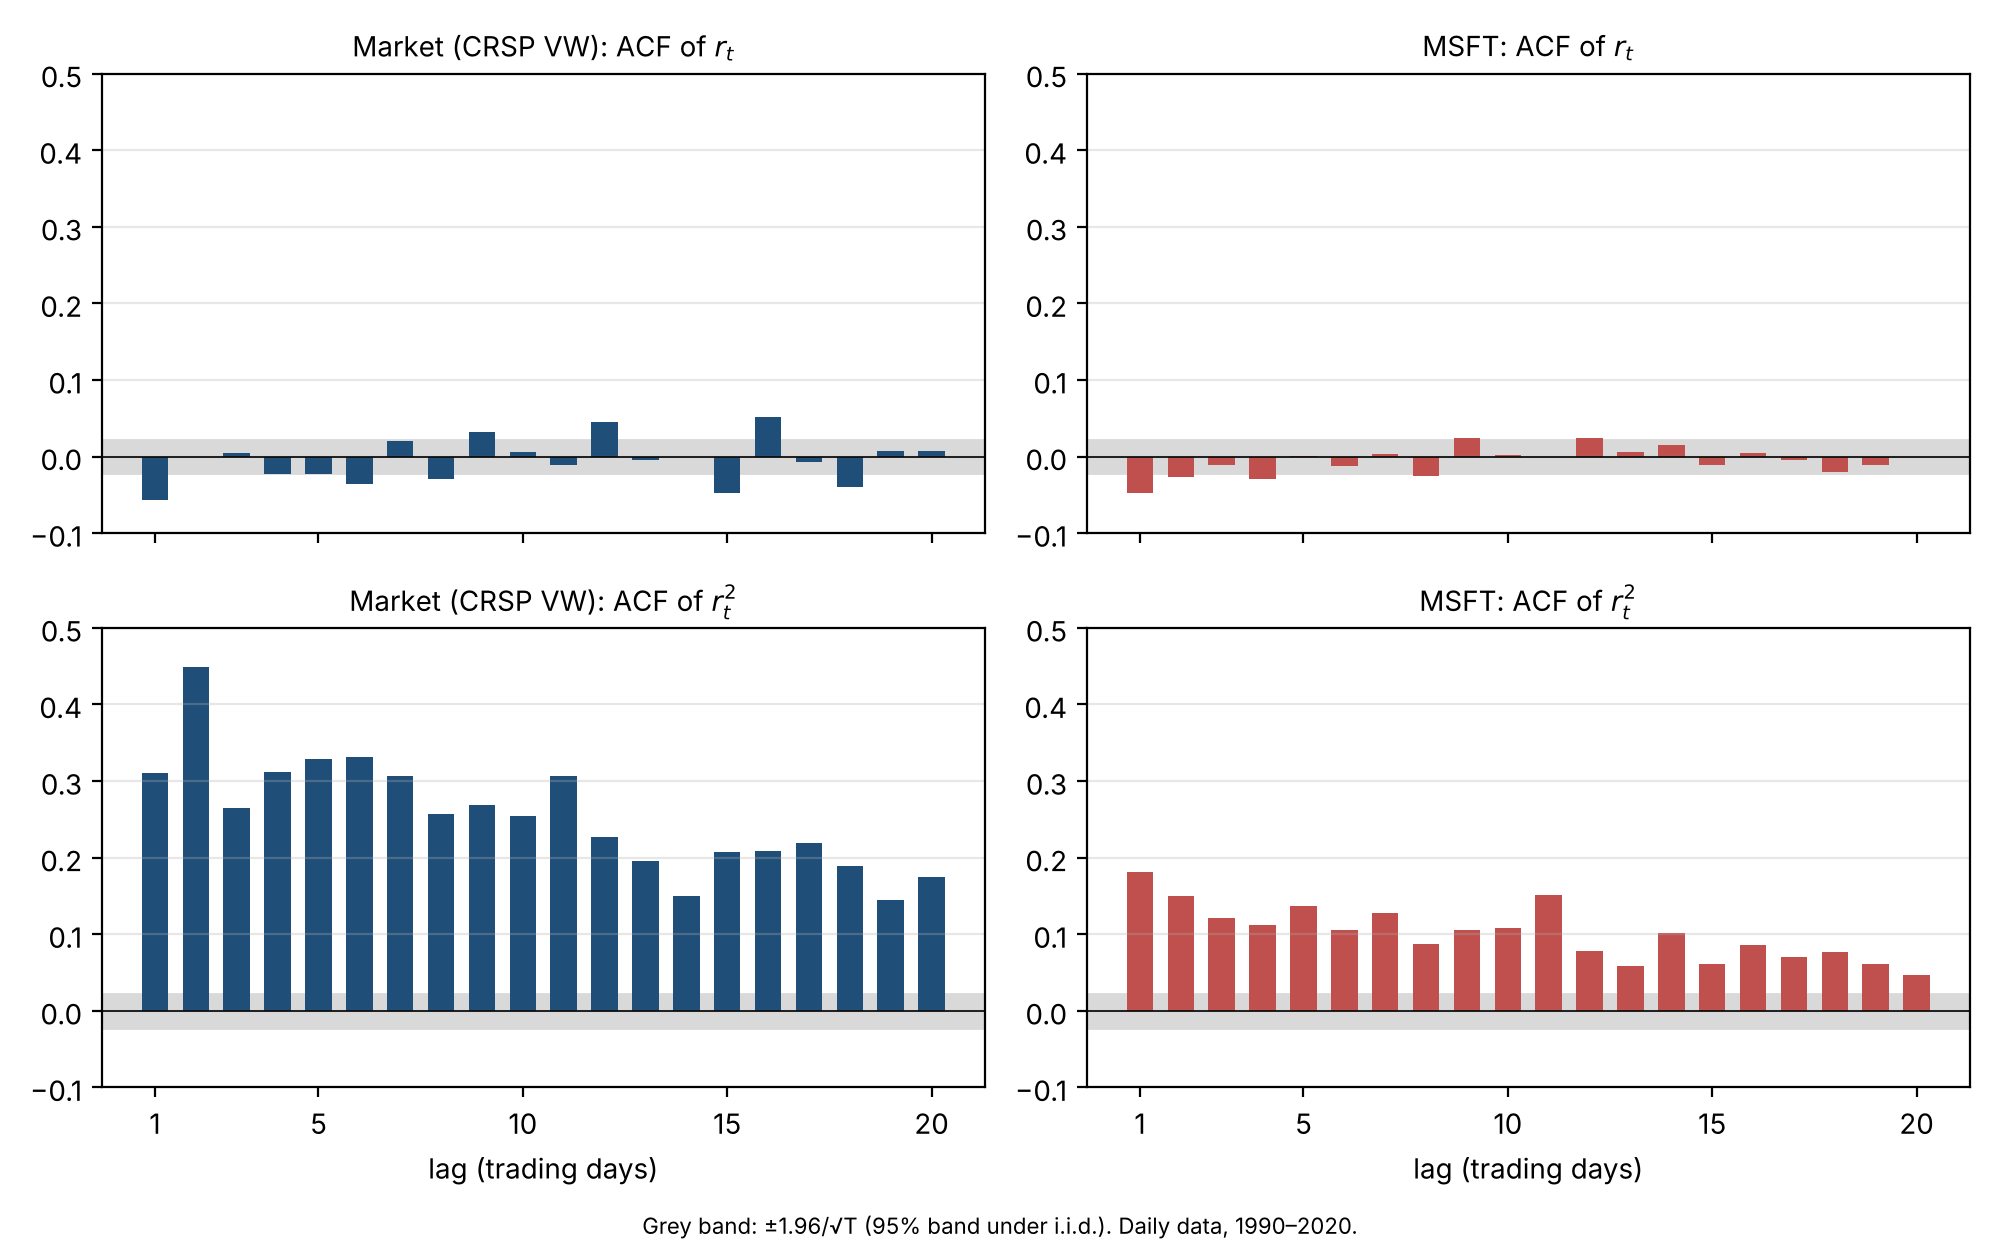
\includegraphics[width=\textwidth]{figures/acf.png}
\caption{Autocorrelations at lags 1--20. Grey band: i.i.d.\ 95\% band $\pm1.96/\sqrt{T}$.
Dashed: heteroskedasticity-robust 95\% band.}
\end{figure}

The data confirm the prior. Squared demeaned returns are positively autocorrelated at all
20 lags in both series, so both show volatility clustering, but the market's clustering is
much stronger. Its autocorrelations average 0.256 over the 20 lags against 0.103 for MSFT,
and its Ljung--Box $Q(20)$ is 11,056 against 1,853. The market's autocorrelations also fade
more slowly, keeping 57\% of their lag-1 value at lag 20 (0.176 against 0.311), while MSFT's
keep 26\% (0.048 against 0.182). The same ordering holds for absolute returns, which are much
less sensitive to a few extreme days, so the result does not come from outliers.

Two further facts support the mechanism behind the prior. First, the firm-specific part of
MSFT's return, the residual from a regression on the market, has squared-return
autocorrelations that average only 0.062. MSFT's autocorrelations sit between that value
and the market's, which is what one would expect if they are a blend of a strongly clustered
market component and a weakly clustered firm component. Second, three of MSFT's five largest
daily moves were firm-specific jumps: $+19.6\%$ on 19 October 2000, $-15.6\%$ on 24 April 2000
and $-14.5\%$ on 3 April 2000, days on which the market moved by less than 4\%. The other two,
$+18.6\%$ on 13 October 2008 and $-14.7\%$ on 16 March 2020, came on days when the market itself
moved by more than 11\%. The unconditional excess kurtosis is higher for the market (11.0
against 6.5), but that is because volatility clustering itself fattens the unconditional tails.
Once the GARCH model in part (b) removes the clustering, the excess kurtosis of the
standardized residuals is 5.8 for MSFT against 1.9 for the market, which is the signature of
jumps that the volatility state does not predict.

The return autocorrelations are small, as expected. None exceeds 0.06 in absolute value.
Against the usual $\pm1.96/\sqrt{T}$ band, 10 of the market's 20 lags and 6 of MSFT's look
significant, but that band assumes constant variance and is too narrow here. With a band that
allows for time-varying variance, 4 market lags and 1 MSFT lag remain significant, and the
largest coefficient, $-0.056$ for the market at lag 1, implies that less than 0.4\% of the
return variance is predictable from the previous day.

\subsection{(b) Gaussian GARCH(1,1) by maximum likelihood}

The model is
\[
r_t = \mu + \varepsilon_t,\qquad \varepsilon_t=\sigma_t z_t,\quad z_t \overset{iid}{\sim} N(0,1),\qquad
\sigma_t^2 = \omega + \alpha\,\varepsilon_{t-1}^2 + \beta\,\sigma_{t-1}^2,
\]
with $\omega>0$, $\alpha,\beta\ge0$ and $\alpha+\beta<1$. Conditional on $\mathcal F_{t-1}$,
$r_t\sim N(\mu,\sigma_t^2)$ and $\sigma_t^2$ is a known function of $\theta=(\mu,\omega,\alpha,\beta)$
and past returns. The log likelihood is therefore the sum of the one-step conditional
normal log densities,
\[
\mathcal L(\theta) = -\frac12\sum_{t=1}^{T}\left[\log(2\pi)+\log\sigma_t^2(\theta)+\frac{(r_t-\mu)^2}{\sigma_t^2(\theta)}\right],
\qquad \hat\theta=\arg\max_\theta \mathcal L(\theta),
\]
where the variance recursion starts from $\sigma_1^2 = T^{-1}\sum_t(r_t-\mu)^2$.

\begin{table}[!htb]
\centering
\small
\begin{tabular}{lrrrrrrrr}
\toprule
 & $\mu$ & $\omega$ & $\alpha$ & $\beta$ & $\alpha+\beta$ & Half-life & Long-run vol & $\log L$ \\
\midrule
Market & 0.071 & 0.0175 & 0.112 & 0.873 & 0.985 & 47 & 17.4\% & $-10{,}110.2$ \\
       & (0.009) & (0.0035) & (0.012) & (0.012) & (0.005) & & & \\
MSFT   & 0.116 & 0.066 & 0.079 & 0.906 & 0.985 & 47 & 33.9\% & $-15{,}649.6$ \\
       & (0.018) & (0.036) & (0.025) & (0.030) & (0.009) & & & \\
\bottomrule
\end{tabular}
\caption{GARCH(1,1) estimates; robust s.e.\ in parentheses. The s.e.\ of $\alpha+\beta$ uses
the delta method with the full covariance matrix. Half-life (days) = $\log0.5/\log(\alpha+\beta)$
for deviations of the variance from its long-run level. Long-run vol
= $\sqrt{252\,\omega/(1-\alpha-\beta)}$.}
\end{table}

Both fits have the usual daily-data shape. A return surprise moves next-day variance only
a little ($\alpha$ around 0.1), but the variance remembers its past almost completely
($\beta$ around 0.9), so $\alpha+\beta=0.985$ and a deviation of the variance from its
long-run level takes about 47 trading days to shrink by half. Whether persistence is
significantly below one depends on the standard error of the sum, and that standard error
cannot be read off the two individual ones. The estimates of $\alpha$ and $\beta$ are
strongly negatively correlated ($-0.93$ for the market and $-0.97$ for MSFT), because the
likelihood can trade a higher $\alpha$ against a lower $\beta$ with little change in fit. With
the covariance included, the standard error of $\alpha+\beta$ is 0.0046 for the market and
0.0086 for MSFT. A one-sided test of the integrated null $\alpha+\beta=1$ rejects clearly for
the market ($t=3.2$) and only marginally for MSFT ($t=1.7$, $p\approx0.045$), so MSFT's
long-run variance is estimated much less precisely.

The two series differ in how they reach the same persistence. The market's variance reacts
more to each surprise ($\alpha=0.112$ against 0.079), which is the model's version of its
higher squared-return autocorrelations in part (a), while MSFT relies more on its own lagged
variance. The implied long-run volatilities of 17.4\% and 33.9\% are close to the sample
volatilities of 17.9\% and 32.1\%. On the standardized residuals, $Q(20)$ of the squares falls
to 25.2 ($p=0.19$) for the market and 11.6 ($p=0.93$) for MSFT, so one GARCH(1,1) equation
captures essentially all of the clustering. It does not capture the tails: the
standardized residuals still have excess kurtosis of 1.9 and 5.8, against zero under
normality. The Gaussian likelihood is therefore a quasi-likelihood. The estimates remain
consistent if the mean and variance equations are right, but the classical standard errors
are not valid. The difference is concentrated in the variance parameters: for MSFT's
$\omega$, $\alpha$ and $\beta$ the robust standard errors are 2.7 to 3.0 times the classical
ones, while for $\mu$ the two are almost identical.

\begin{figure}[!htb]
\centering
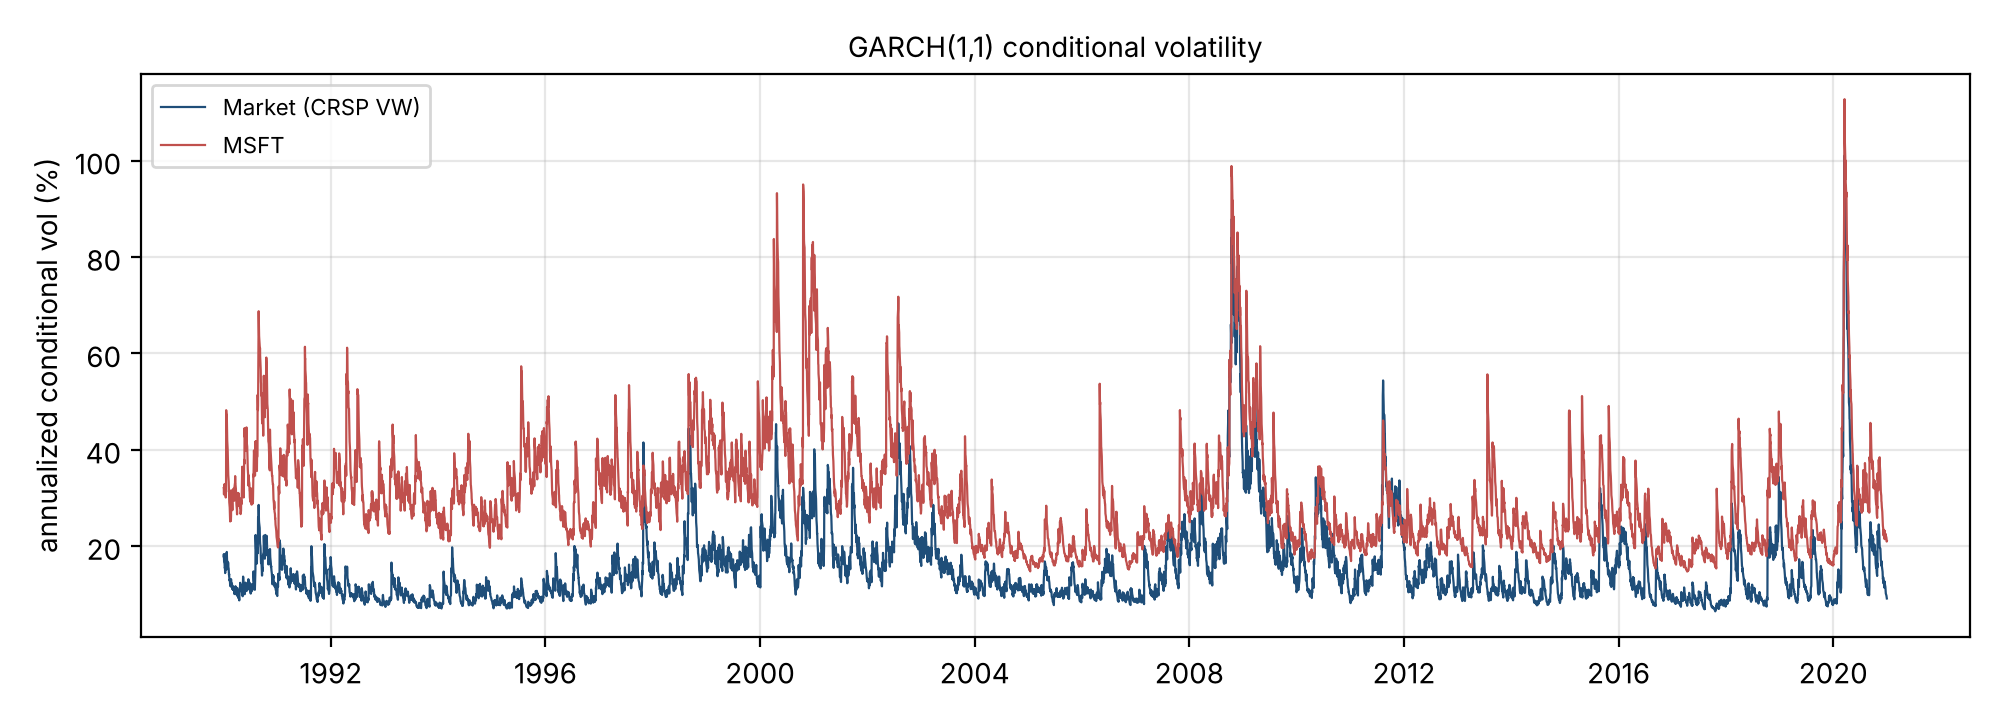
\includegraphics[width=\textwidth]{figures/garch_vol.png}
\caption{GARCH(1,1) conditional volatility, annualized.}
\end{figure}

\subsection{(c) Is MSFT's volatility just the market moving?}

If the risk manager were right, MSFT's conditional variance would be close to
$b^2\sigma^2_{m,t}$, and three things would follow. The market would explain most of MSFT's
return variance, the firm-specific residual would carry no volatility dynamics of its own,
and MSFT's variance would rise and fall one-for-one with the market's. The estimates reject
all three.

The market model $r_{MSFT,t}=a+b\,r_{m,t}+u_t$ gives $\hat b=1.15$ (White s.e.\ 0.021) and
$R^2=0.41$. Over 1990--2020 the market accounts for 41\% of MSFT's daily variance, and the
other 59\% is firm-specific. The residual is also far from noise. A GARCH(1,1) fitted to $u_t$
gives $\alpha=0.024$ (0.006) and $\beta=0.971$ (0.007), with persistence 0.995 (0.002), and
$Q(20)$ of $u_t^2$ is 704. Firm-specific volatility therefore has its own slow-moving state,
at least as persistent as the market's, and a beta-scaled market forecast would miss it
entirely. Finally, a regression of MSFT's fitted log variance on the market's fitted log
variance has a slope of 0.50 and an $R^2$ of 0.39. Under the claim both would be close to one.
A doubling of market variance is associated with roughly a 40\% rise in MSFT's variance, and
most of the movement in MSFT's variance is unrelated to the market's.

The two GARCH fits also show when the claim comes closest to holding. Combining them gives
an approximate market-related share of MSFT's variance,
\[
s_t=\frac{b^2\hat\sigma^2_{m,t}}{b^2\hat\sigma^2_{m,t}+\hat\sigma^2_{u,t}} .
\]
This is an approximation, not an exact conditional decomposition, because it assumes a
constant beta and a market return that is conditionally uncorrelated with $u_t$. OLS only
guarantees zero correlation on average, and yearly betas range from 0.73 to 2.30. As a check,
the implied total variance averages 1.05 times MSFT's own GARCH variance, with a 10th--90th
percentile range of 0.72 to 1.43. The share averages 0.36 and exceeds one half on only 20\% of
days.

\begin{table}[!htb]
\centering
\small
\begin{tabular}{lrrr}
\toprule
Period & Approx.\ market share & Market-related vol & Firm-specific vol \\
\midrule
Full sample 1990--2020 & 0.36 & 17.8\% & 23.5\% \\
Dot-com and antitrust 2000--02 & 0.36 & 25.3\% & 33.8\% \\
Financial crisis Sep 2008--Jun 2009 & 0.64 & 49.4\% & 33.7\% \\
COVID crash Mar--Apr 2020 & 0.87 & 71.3\% & 24.2\% \\
Calm year 2017 & 0.32 & 10.0\% & 14.7\% \\
\bottomrule
\end{tabular}
\caption{Average approximate market-related share of MSFT's conditional variance, and the
average annualized volatility of each part.}
\end{table}

The share is high only in market-wide crises. In the 2008--09 financial crisis it averaged
0.64 and in March--April 2020 it reached 0.87, because market volatility exploded while
MSFT's firm-specific volatility rose much less. In those months the risk manager's
description is roughly right. In calm markets it is wrong (0.32 in 2017), and in 2000--02 it
is wrong for the opposite reason: MSFT's volatility was very high, but the antitrust case and
the end of the technology boom raised its firm-specific volatility (33.8\%) as much as its
market-related volatility, so the share stayed at its average. The relationship has tightened
in recent years, with a yearly $R^2$ of 0.64 to 0.75 in 2018--2020, as Microsoft became one of
the largest weights in the index. Taken over the whole sample, though, most of MSFT's risk is
its own, and a risk model that treats MSFT as leveraged market exposure would understate its
risk in normal times and miss firm-specific episodes altogether.

\begin{figure}[!htb]
\centering
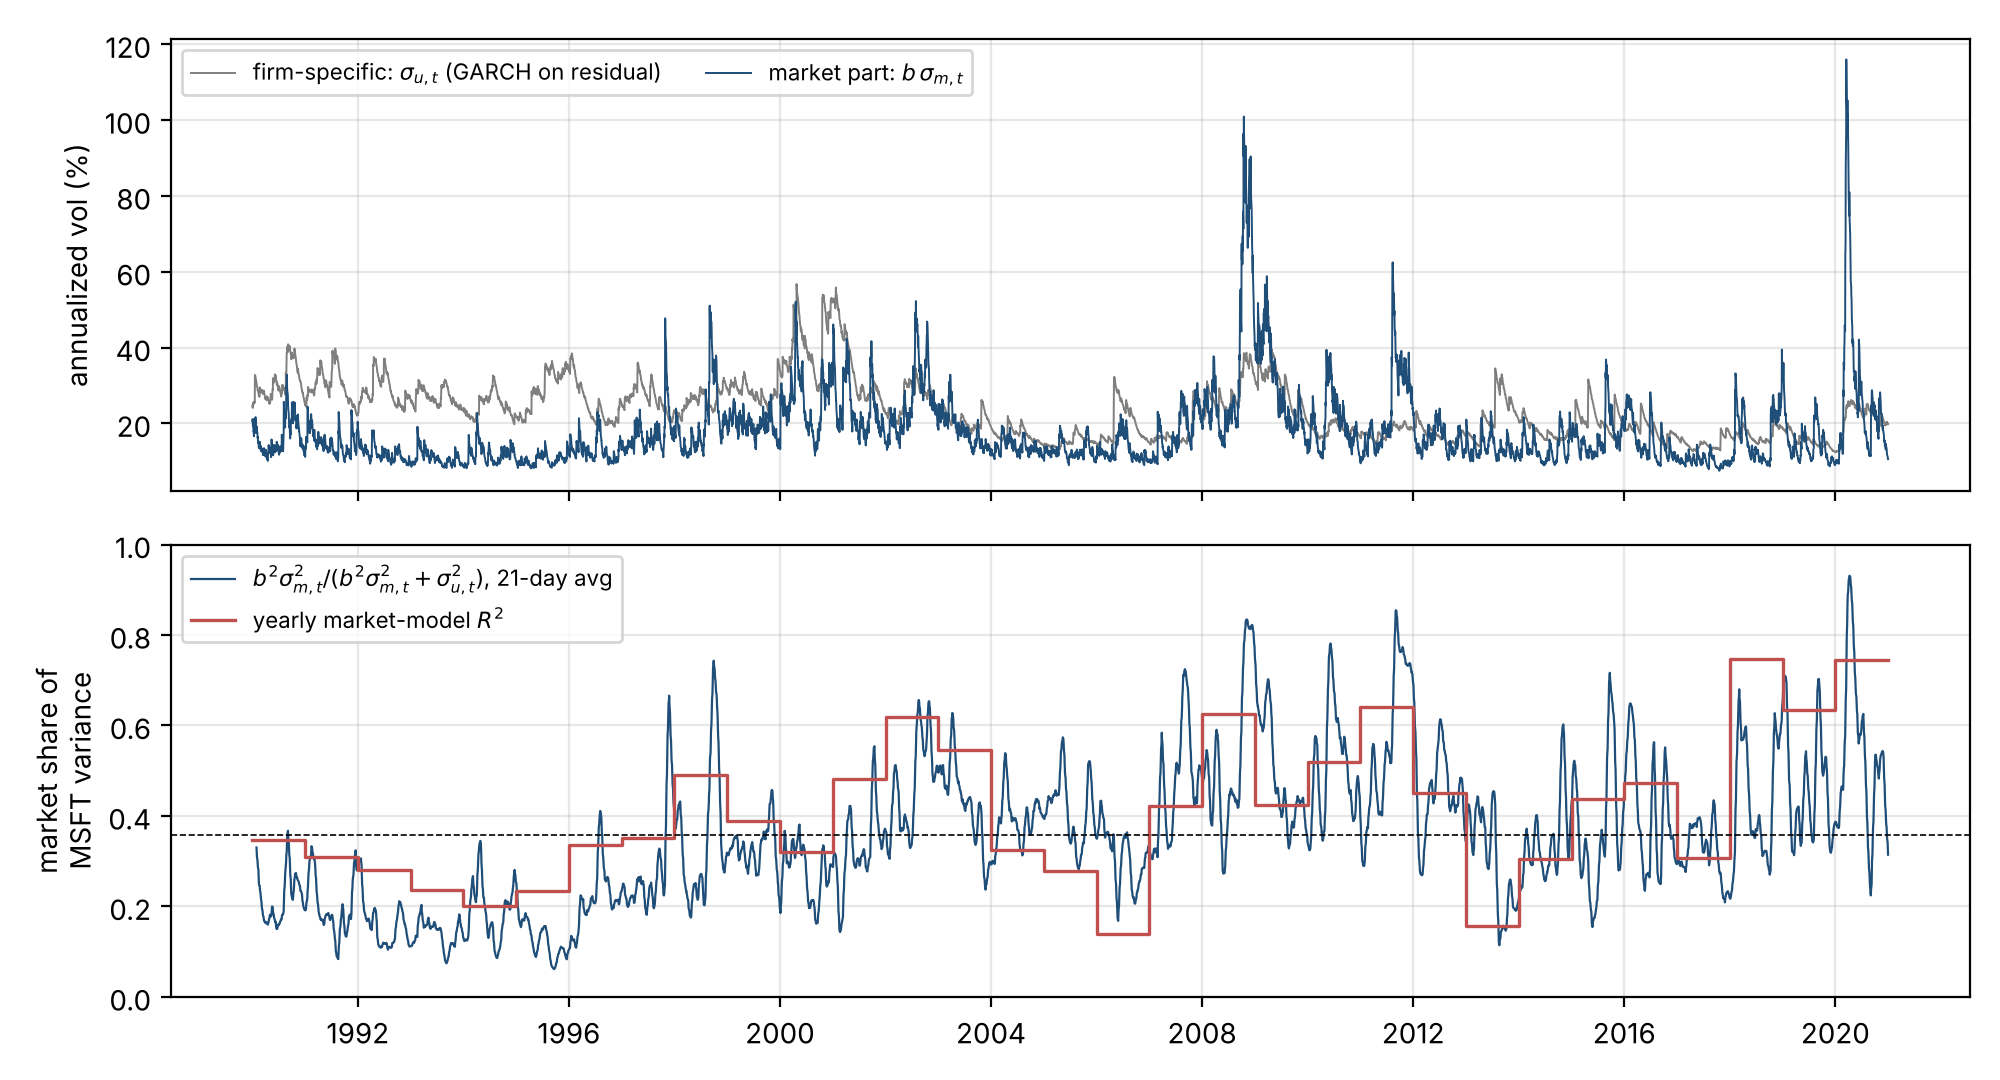
\includegraphics[width=\textwidth]{figures/msft_decomp.png}
\caption{Top: market-related ($b\,\sigma_{m,t}$) and firm-specific ($\sigma_{u,t}$)
volatility of MSFT. Bottom: approximate market-related share of MSFT's variance (dashed: mean)
and yearly market-model $R^2$.}
\end{figure}

\subsection{(d) Market risk over the next month (as of 31 December 2020)}

The forecasts come from the fitted GARCH(1,1) for the market. The variance forecast $h$ days
ahead is $\E_t\sigma^2_{t+h}=\bar\sigma^2+(\alpha+\beta)^{h-1}(\sigma^2_{t+1}-\bar\sigma^2)$,
so a gap between today's variance and its long-run level halves in about 47 trading days. The
one-month variance is the sum of the 21 daily forecasts, which gives a one-month standard
deviation of 3.0\% against 5.0\% at the long-run level. The ranges and loss probabilities below
come from 200,000 simulated 21-day paths of the fitted model, because a month of GARCH returns
is not exactly normal. They set the expected return to zero; the fitted mean of 0.071\% a day,
about 18\% a year, would shift every figure up by 1.5 percentage points. For a reader who has
never heard of GARCH, the model says three things.

\begin{itemize}
\item Risk is low right now. Recent daily moves have been small, so the model puts the
market's volatility at about 9\% a year, half its long-run level of 17\%. Calm periods tend to
last.
\item It will rise only slowly. Volatility drifts back toward normal over several months and
reaches only about 12\% by the end of January. A typical month should move the market about
3\% up or down, against 5\% normally, and 19 months in 20 like this one end between $-6\%$ and
$+6\%$.
\item A bad month is still possible. About 1 month in 100 like this one loses more than
7.5\%, and one large shock would raise all of these numbers at once: in March 2020 the same
model put volatility near 100\%. Real crashes are also more likely than the model's bell-curve
shocks allow.
\end{itemize}

%=====================================================================
\section{Question 2 (PhD): Gaussian GARCH-in-mean}

In the GARCH-in-mean model the conditional variance enters the expected return,
$r_t=\mu+\lambda\,g(\sigma_t^2)+\varepsilon_t$ with $\varepsilon_t=\sigma_tz_t$,
$z_t\sim N(0,1)$ and $\sigma_t^2=\omega+\alpha\varepsilon_{t-1}^2+\beta\sigma_{t-1}^2$, where
$g(\sigma^2)$ is usually $\sigma^2$, $\sigma$ or $\log\sigma^2$. The MLE solves
\[
\hat\theta=\arg\max_{\theta}\; -\frac12\sum_{t=1}^T\left[\log2\pi+\log\sigma_t^2(\theta)
+\frac{\big(r_t-\mu-\lambda g(\sigma_t^2(\theta))\big)^2}{\sigma_t^2(\theta)}\right]
\quad\text{s.t. } \omega>0,\ \alpha,\beta\ge0,\ \alpha+\beta<1 .
\]
The difference from plain GARCH is that the residual $\varepsilon_t=r_t-\mu-\lambda
g(\sigma_t^2)$ now depends on the variance parameters, so the mean and variance recursions
have to be run together: $\sigma_t^2$ is built from $\varepsilon_{t-1}$, and $\varepsilon_t$
is then built from $\sigma_t^2$. For the same reason the information matrix is no longer
block-diagonal between mean and variance parameters. A misspecified variance equation now
biases the estimate of $\lambda$, and the two blocks cannot be estimated in separate steps.
Because a misspecified variance equation biases $\lambda$, the estimate should come from a
variance equation the data support. The table below estimates the model with
$g(\sigma^2)=\sigma^2$ under each of the variance equations compared in Question 3.

\begin{table}[!htb]
\centering
\small
\begin{tabular}{lrrr}
\toprule
Variance equation & Market $\hat\lambda$ & MSFT $\hat\lambda$ & CAPM benchmark for MSFT \\
\midrule
GARCH-$N$ & 0.041 (0.013) & 0.012 (0.009) & 0.015 \\
GARCH-$t$ & 0.034 (0.012) & 0.005 (0.007) & 0.012 \\
GJR-$N$   & 0.021 (0.011) & 0.008 (0.009) & 0.008 \\
GJR-$t$   & 0.023 (0.010) & 0.004 (0.007)$^\dagger$ & 0.008 \\
\bottomrule
\end{tabular}
\caption{GARCH-in-mean estimates of $\lambda$ with $g(\sigma^2)=\sigma^2$; robust s.e.\ in
parentheses. The CAPM benchmark is $\lambda_m R^2/b$ with the market $\hat\lambda$ from the
same row. $^\dagger$MSFT's variance persistence is on the imposed bound, so this s.e.\ is only
indicative.}
\label{tab:garchm}
\end{table}

For the market, adding the leverage term roughly halves $\hat\lambda$, from 0.041 under the
symmetric Gaussian GARCH to 0.023 (0.010) under GJR-$t$, the specification Question 3 favors.
Which days count as high-variance depends on the variance equation, and $\lambda$ is estimated
from the returns on those days, so the bias described above is large in these data. The
risk--return trade-off stays positive and is marginally significant under GJR-$t$ ($t=2.4$), so
the conclusion survives, but it is about half as strong as the symmetric model suggests. This
is the problem the GJR model was introduced to address; in its first application, allowing for
asymmetric volatility turned the estimated risk--return relation negative.

For MSFT, $\hat\lambda$ is small and insignificant under every variance equation, and each
estimate is within one standard error of what CAPM implies. If only market risk is priced,
MSFT's premium is $b\,\lambda_m\sigma^2_{m,t}$, so its price per unit of total variance should
be $\lambda_m R^2/b$: 0.015 under the Gaussian GARCH and 0.008 under GJR-$t$, against estimates
of 0.012 and 0.004. MSFT's $\lambda$ is lower than the market's because most of its variance is
firm-specific and earns no premium.

Additional return predictors enter the mean equation. With
$m_t=\mu+\lambda g(\sigma_t^2)+\gamma'X_{t-1}$ the objective is unchanged except that
$\varepsilon_t=r_t-m_t$, and the variance recursion is fed this new residual. The predictors
must be known at $t-1$, and they must not be collinear with $g(\sigma_t^2)$. If one of them is
itself a volatility proxy, such as a lagged VIX, $\lambda$ and $\gamma$ are only weakly
identified.

Variance predictors enter the GARCH equation,
$\sigma_t^2=\omega+\alpha\varepsilon_{t-1}^2+\beta\sigma_{t-1}^2+\delta'Q_{t-1}$, again with
the same objective, but the restrictions that make plain GARCH well behaved no longer cover
the new term. The first problem is positivity. The conditions $\omega>0$ and $\alpha,\beta\ge0$
guarantee $\sigma_t^2>0$ in plain GARCH, but $\delta'Q_{t-1}$ can be negative, and a single
negative variance makes the likelihood undefined. The simplest fix is to use non-negative
predictors, such as variances or squared spreads, together with $\delta\ge0$. For predictors
of either sign one has to restrict $\omega+\delta'Q_t>0$ over the support of $Q$ or
reparametrize, for example with $\exp(\delta'Q_{t-1})$ or an EGARCH-X model for
$\log\sigma_t^2$. The predictors must also be predetermined, $Q_{t-1}\in\mathcal F_{t-1}$;
otherwise $\sigma_t^2$ is no longer a conditional variance and the prediction-error
decomposition behind the likelihood breaks down.

The second problem is stationarity. With an exogenous input, $\alpha+\beta<1$ is no longer
enough, because the variance inherits the behaviour of $Q$. $Q_t$ must be strictly stationary
and ergodic with $\E|Q_t|<\infty$, in which case
$\E\sigma^2=(\omega+\delta'\E Q)/(1-\alpha-\beta)$; a trending or unit-root predictor would
make $\sigma_t^2$ non-stationary however small $\alpha+\beta$ is. These conditions, together
with identification, give consistency of the (Q)MLE. Asymptotic normality needs more: an
interior true parameter, $\E z_t^4<\infty$ so that the score has finite variance, and enough
moments of $Q_t$ and $\sigma_t^2$ for the score and Hessian to obey a law of large numbers and a
central limit theorem. Identification
requires that $Q$ vary over time and not be collinear with $\varepsilon_{t-1}^2$ or
$\sigma_{t-1}^2$, since otherwise $\omega$, $\delta$ and $\beta$ cannot be separated. Finally,
the sign restriction matters for testing. If $\delta\ge0$ is imposed, $\delta=0$ lies on the
boundary of the parameter space, and for a scalar $\delta$ with the other parameters interior
the likelihood-ratio statistic converges to $\tfrac12\chi^2_0+\tfrac12\chi^2_1$ rather than
$\chi^2_1$.

%=====================================================================
\section{\texorpdfstring{Question 3 (PhD): GJR-GARCH(1,1,1) with Student-$t$ innovations}{Question 3 (PhD): GJR-GARCH(1,1,1) with Student-t innovations}}

The model is $r_t=\mu+\varepsilon_t$, $\varepsilon_t=\sigma_tz_t$, with $z_t$ i.i.d.\
standardized Student-$t$ (mean 0, variance 1, $\nu>2$) and
\[
\sigma_t^2=\omega+\big(\alpha+\gamma\,\1\{\varepsilon_{t-1}<0\}\big)\varepsilon_{t-1}^2+\beta\sigma_{t-1}^2 ,
\]
so a negative return raises next-day variance by $\alpha+\gamma$ per unit of squared return
and a positive return by $\alpha$. The log likelihood is
\[
\mathcal L=\sum_t\left[\log\Gamma\!\left(\tfrac{\nu+1}{2}\right)-\log\Gamma\!\left(\tfrac{\nu}{2}\right)
-\tfrac12\log\big(\pi(\nu-2)\big)-\tfrac12\log\sigma_t^2
-\tfrac{\nu+1}{2}\log\!\left(1+\frac{\varepsilon_t^2}{(\nu-2)\sigma_t^2}\right)\right].
\]

To derive the non-integration condition, substitute $\varepsilon_{t-1}^2=\sigma_{t-1}^2z_{t-1}^2$
and note that $\1\{\varepsilon_{t-1}<0\}=\1\{z_{t-1}<0\}$ because $\sigma_{t-1}>0$:
\[
\sigma_t^2=\omega+\sigma_{t-1}^2\big[\alpha z_{t-1}^2+\gamma z_{t-1}^2\1\{z_{t-1}<0\}+\beta\big].
\]
$z_{t-1}$ is independent of $\sigma_{t-1}^2\in\mathcal F_{t-2}$ and $\E z^2=1$. Let
$\kappa=\E[z^2\1\{z<0\}]$ be the part of $\E z^2$ that comes from negative shocks. Taking
expectations at $t-2$,
\[
\E_{t-2}\sigma_t^2=\omega+\phi\,\sigma_{t-1}^2,\qquad \phi=\alpha+\kappa\gamma+\beta .
\]
The model assumes a standardized $t$, which is symmetric about zero, so $\kappa=\tfrac12$ and
$\phi=\alpha+\tfrac12\gamma+\beta$. Iterating gives
$\E_{t-k}\sigma_t^2=\omega\sum_{j=0}^{k-2}\phi^j+\phi^{k-1}\sigma_{t-k+1}^2$. The effect of
today's variance on the forecast $k$ periods ahead decays like $\phi^{k}$, and the
unconditional variance $\E\varepsilon_t^2=\omega/(1-\phi)$ is finite if and only if
\[
\boxed{\ \alpha+\tfrac12\gamma+\beta<1\ }
\qquad(\omega>0,\ \alpha\ge0,\ \alpha+\gamma\ge0,\ \beta\ge0,\ \nu>2).
\]
At $\phi=1$ the variance is integrated: a shock never dies out of the variance forecast, and
the unconditional variance is infinite. This does not mean volatility explodes. Strict
stationarity only requires $\E\log(\alpha z^2+\gamma z^2\1\{z<0\}+\beta)<0$, and at $\phi=1$
this holds by Jensen's inequality, since $\E\log X<\log\E X=0$ for any non-degenerate $X$. An
integrated GJR process can therefore be strictly stationary, and the effect of a shock on
future variance still dies out with probability one even though its effect on the expected
variance does not.

\begin{table}[!htb]
\centering
\small
\begin{tabular}{lrrrrrrrr}
\toprule
 & $\mu$ & $\omega$ & $\alpha$ & $\gamma$ & $\beta$ & $\nu$ & $\phi$ & $\log L$ \\
\midrule
Market & 0.065 & 0.0137 & 0.009 & 0.163 & 0.895 & 6.9 & 0.985 & $-9{,}832.4$ \\
       & (0.008) & (0.0024) & (0.006) & (0.018) & (0.010) & (0.57) & (0.003) & \\
MSFT$^\dagger$ & 0.073 & 0.032 & 0.056 & 0.068 & 0.910 & 5.3 & 0.99999 & $-15{,}220.2$ \\
       & (0.016) & (0.010) & (0.010) & (0.015) & (0.014) & (0.32) & -- & \\
\bottomrule
\end{tabular}
\caption{GJR-GARCH-$t$ estimates; robust s.e.\ in parentheses. $\phi=\alpha+\gamma/2+\beta$
uses the model's symmetry assumption; with the sample weight on negative shocks
($\hat\kappa=0.583$ for the market) the market's $\phi$ is 0.999.
$^\dagger$The constraint $\phi\le1-10^{-5}$ imposed in estimation binds for MSFT
($\hat\phi=0.99999$). Without it $\hat\phi=1.0017$ with a log-likelihood gain of 0.12
(LR = 0.24). The MSFT standard errors are computed as if the estimate were interior and are
only indicative.}
\end{table}

\begin{table}[!htb]
\centering
\small
\begin{tabular}{lrrrr}
\toprule
 & GARCH-$N$ & GARCH-$t$ & GJR-$N$ & GJR-$t$ \\
\midrule
Market & $-10{,}110.2$ & $-9{,}927.3$ & $-9{,}999.7$ & $-9{,}832.4$ \\
MSFT & $-15{,}649.6$ & $-15{,}238.3$ & $-15{,}624.5$ & $-15{,}220.2$ \\
\bottomrule
\end{tabular}
\caption{Log likelihood by model, showing how much fat tails and leverage each add. All four
likelihoods are coded by hand and use the same variance initialization.}
\end{table}

Relative to the Gaussian GARCH(1,1), GJR-$t$ raises the log likelihood by 278 for the market
and 429 for MSFT, far more than two extra parameters could produce by chance. The second
table shows where the gain comes from. Fat tails matter for both series ($\hat\nu=6.9$ and
5.3; switching to $t$ errors alone adds 183 and 411), and they matter most for MSFT, whose
firm-specific jumps are exactly the extreme standardized shocks a normal distribution cannot
produce. Leverage matters a great deal for the market (it adds 110) and little for MSFT (25).

The parameters move in ways that follow from this. For the market, the symmetric coefficient
falls from 0.112 to an insignificant 0.009 and the asymmetry term $\gamma=0.163$ takes over,
so the GARCH(1,1) $\alpha$ was an average of a strong response to bad news and almost no
response to good news. Under the model's symmetry assumption the market's persistence is
$\phi=0.985$ (s.e.\ 0.0035), apparently well below one, with an implied long-run volatility of
15.2\%. Both numbers rest on negative shocks carrying half of $\E z^2$, and the data reject
that. The market's standardized residuals are negatively skewed (skewness $-0.59$), and
negative shocks carry 58.3\% (approximate s.e.\ 1.2\%) of their squared mass. Because the
market's $\gamma$ is large, the difference matters: with the sample weight, $\phi=0.9987$
(approximate s.e.\ 0.0041), which is not significantly below one. This standard error is a
plug-in calculation that ignores the covariance between the fitted parameters and the
estimated weight. Within one standard error $\phi$ reaches one, so the implied long-run
volatility ranges from about 25\% a year to infinity and is no longer pinned down. The GJR-$t$ fit should therefore not be used for the market's long-run
volatility level. The GARCH(1,1) estimate of 17.4\%, close to the sample's 17.9\%, is the
better guide, and a skewed-$t$ density would be the natural next step. For MSFT persistence
rises to the bound $\phi\le1-10^{-5}$. Under $t$ errors the largest
firm-specific moves are treated as draws from a fat tail, so they no longer pull $\beta$ down,
and the fitted variance becomes smoother and more persistent. Dropping the bound gives
$\hat\phi=1.0017$ with a log-likelihood gain of only 0.12, so the data cannot distinguish
MSFT's variance in this model from an integrated process. Its long-run variance is infinite at
the unconstrained estimate and cannot be estimated reliably, and its standard errors rest on
interior asymptotics that do not apply at the boundary. MSFT's residuals are close to
symmetric ($\hat\kappa=0.47$), so this conclusion does not depend on the symmetry assumption.

The leverage effect is far stronger for the market. Bad news raises the market's next-day
variance 19 times as much as good news of the same size ($\alpha+\gamma=0.171$ against
$\alpha=0.009$), while for MSFT the ratio is 2.2 (0.124 against 0.056). This is hard to
reconcile with the financial-leverage explanation, in which a falling stock price raises the
debt-to-equity ratio and therefore equity volatility. Microsoft had no
long-term debt until 2009 and little relative to its market value afterwards, yet the
asymmetry is weak for MSFT and very strong for the index. A systematic channel fits better.
Under volatility feedback, news that raises expected market
volatility raises required returns and pushes prices down at the same moment, and
correlations across stocks rise in selloffs, so falling prices and rising volatility arrive
together in the aggregate. Volatility feedback requires a positive price of risk, and
Question 2 finds one under the GJR-$t$ variance equation ($\hat\lambda=0.023$, s.e.\ 0.010). Firm-specific news works differently, because a large earnings surprise
raises uncertainty about the firm whether it is good or bad. In the fitted model, the
$+19.6\%$ move on 19 October 2000 lifted MSFT's annualized volatility from 47\% to 86\% the
next day. Fitting the same GJR-$t$ model to MSFT's market-model residual
makes the point directly: the firm-specific asymmetry is $\gamma=0.017$ (s.e.\ 0.023),
indistinguishable from zero. MSFT's own $\gamma$ is 0.42 times the market's, close to the
0.36--0.41 share of its variance that is market-related, so its asymmetry comes almost entirely
through its market exposure.

\begin{figure}[!htb]
\centering
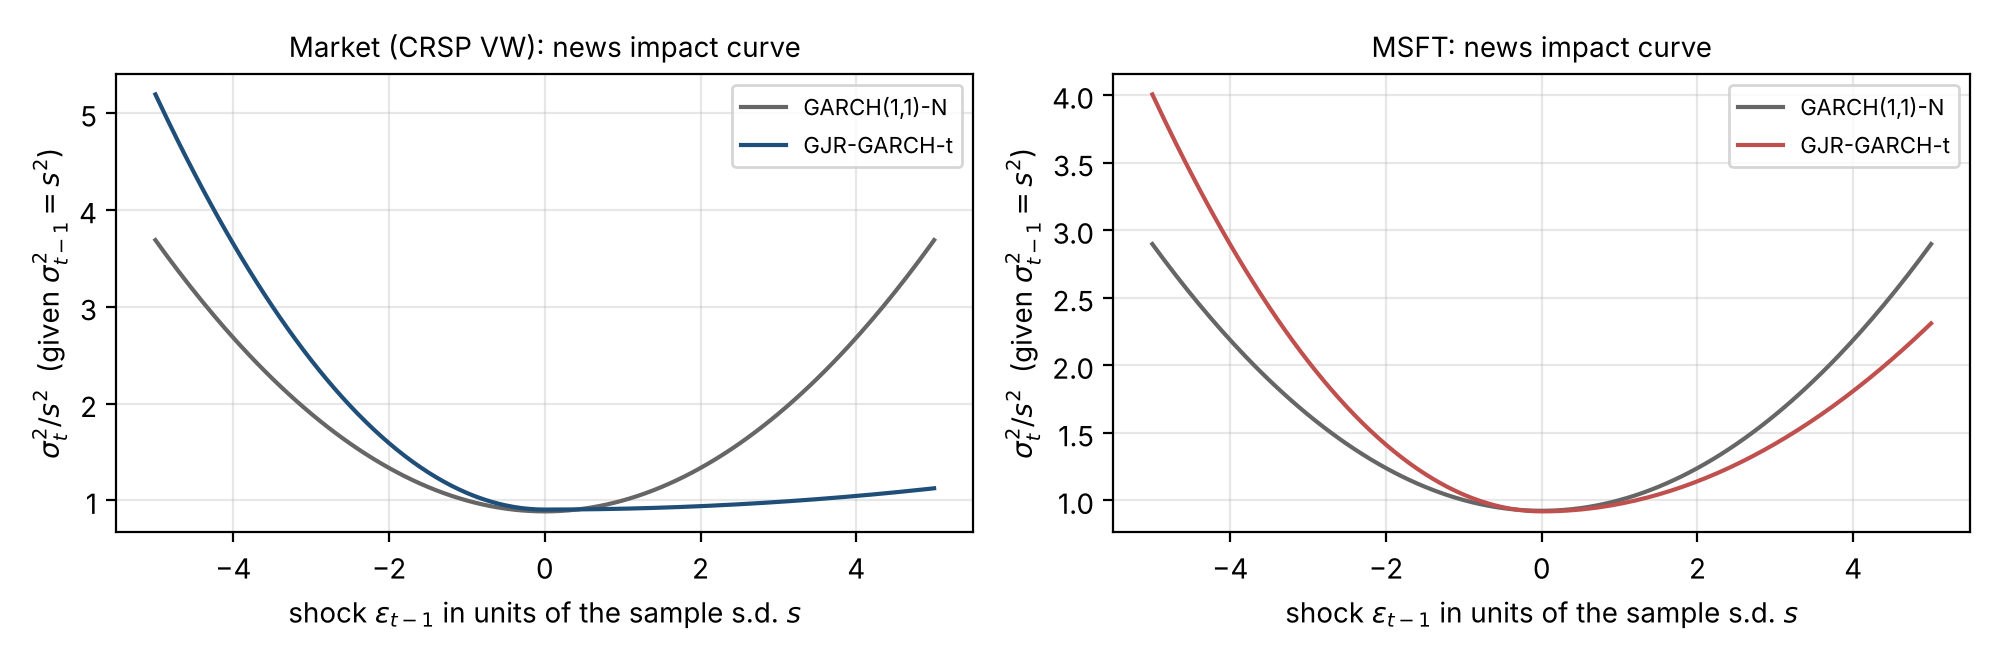
\includegraphics[width=\textwidth]{figures/news_impact.png}
\caption{News impact curves: next-day variance after a shock $\varepsilon_{t-1}$, given that
the previous variance equals the sample variance $s^2$. Axes are scaled by the sample s.d.\
because the long-run variance does not exist for MSFT's GJR-$t$ estimate.}
\end{figure}

\end{document}
